\documentclass[10pt, aspectratio=1610]{beamer}
\usepackage[utf8]{inputenc}
\usepackage[T1]{fontenc}
\usepackage[french]{babel}
\usepackage{amsmath}
\usepackage{amssymb}
\usepackage{graphicx}
\usepackage{booktabs}
\usepackage[utf8]{inputenc}
\usepackage[T1]{fontenc}
\usepackage[french]{babel}
\usepackage{graphicx}
\usepackage{geometry}
\usepackage{float}
\usepackage{amsmath}
\usepackage{amssymb}
\usepackage{hyperref}
\usepackage{xcolor}
\usepackage[most]{tcolorbox} % Pour les beaux encadrés mathématiques
\usepackage{setspace} % Pour aérer le texte

% Thème épuré et professionnel
\usetheme{Boadilla}
\usecolortheme{seahorse}
\setbeamertemplate{navigation symbols}{}
\setbeamertemplate{itemize items}[circle]

% Définition des couleurs pour les encadrés
\definecolor{thmblue}{RGB}{230, 240, 255}
\definecolor{borderblue}{RGB}{0, 80, 160}
\definecolor{defgray}{RGB}{245, 245, 245}
\definecolor{bordergray}{RGB}{100, 100, 100}

\title[Extrêmes COVID-19 (EVT-CART)]{Modélisation Spatiale des Extrêmes de Mortalité COVID-19 aux États-Unis}
\subtitle{De la théorie des valeurs extrêmes à l'outil d'aide à la décision}
\author[Équipe IMI]{Eliott Delhaye, Chloé Spittael, Camille Viénot, Paul-Emile Marcus}
\institute[ENPC]{École Nationale des Ponts et Chaussées}
\date{Soutenance de Projet - 2025/2026}

\begin{document}

% ---------------------------------------------------
% SLIDE 1 : TITRE
% ---------------------------------------------------
\begin{frame}
    \titlepage
\end{frame}

% ---------------------------------------------------
% SLIDE 2 : LE BESOIN OPÉRATIONNEL
% ---------------------------------------------------
\begin{frame}{Le Constat : Anticiper le pire, pas la moyenne}
    \textbf{Le problème des modèles classiques}
    \begin{itemize}
        \item L'analyse épidémiologique standard modélise la \textbf{tendance centrale}.
        \item Lors d'un choc systémique (pandémie), le système de santé ne sature pas à cause de la moyenne, mais à cause des \textbf{valeurs extrêmes} (queues de distribution).
    \end{itemize}
    \vspace{0.4cm}
    
    \begin{alertblock}{La question centrale pour un décideur}
    Comment cartographier rigoureusement le risque de surmortalité extrême en tenant compte des immenses disparités locales (densité, âge, pauvreté) du territoire américain ?
    \end{alertblock}
\end{frame}



% ---------------------------------------------------
% SLIDE 3 : CAS D'USAGE
% ---------------------------------------------------
\begin{frame}{Cas d'Usage : Pourquoi et pour qui ?}
    Notre modélisation s'adresse directement aux planificateurs stratégiques :
    \vspace{0.4cm}

    \begin{columns}
        \begin{column}{0.48\textwidth}
            \textbf{1. Autorités de Santé Publique}
            \begin{itemize}
                \item \textit{Objectif :} Dimensionnement préventif.
                \item Identifier si une région a un "plafond" physique de mortalité ou si le risque est explosif.
                \item Cibler l'allocation des lits de réanimation d'urgence.
            \end{itemize}
        \end{column}
        \begin{column}{0.48\textwidth}
            \textbf{2. Secteur de l'Assurance / Réassurance}
            \begin{itemize}
                \item \textit{Objectif :} Solvabilité.
                \item Estimer la probabilité d'événements hors de l'échantillon historique.
                \item Calculer une \textit{Value-at-Risk} (VaR) territorialisée pour provisionner le risque pandémique.
            \end{itemize}
        \end{column}
    \end{columns}
\end{frame}


% ---------------------------------------------------
% SLIDE 11 : LA CARTE FINALE
% ---------------------------------------------------
\begin{frame}[plain]{Livrable Décideur : Cartographie du Risque Extrême ($\xi$)}
    \begin{center}
        \vfill
        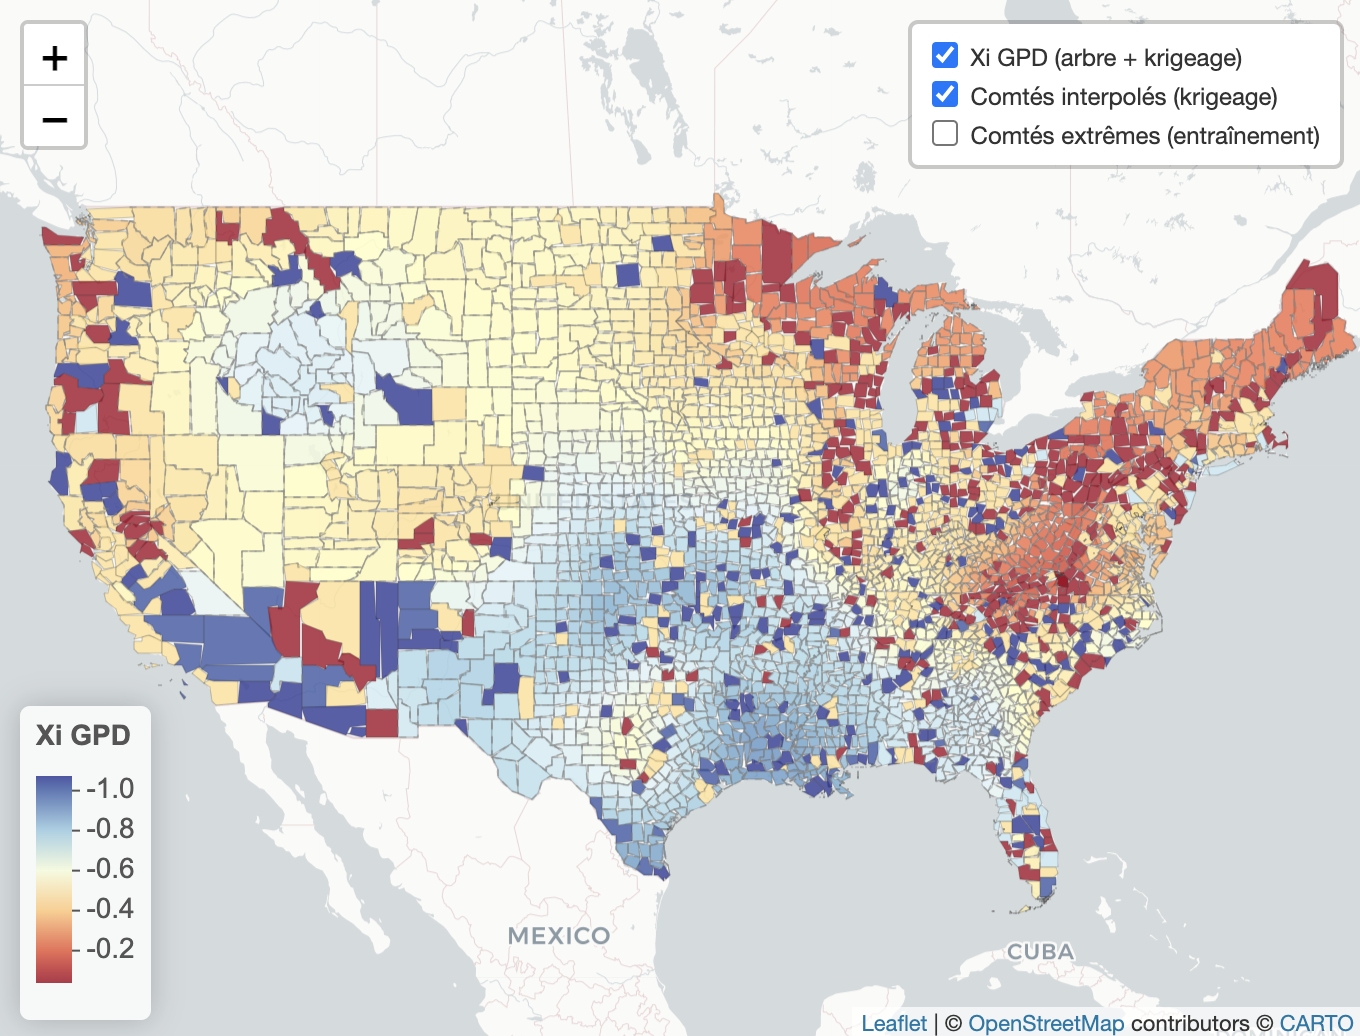
\includegraphics[width=0.9\textwidth, height=0.85\textheight, keepaspectratio]{carte1.png}
        \vfill
    \end{center}
\end{frame}
% ---------------------------------------------------
% SLIDE 4 : LA THEORIE
% ---------------------------------------------------
\begin{frame}{Le socle mathématique : Théorie des Valeurs Extrêmes}
    Pour inférer au-delà des données observées, nous utilisons l'approche \textbf{Peaks over Threshold (PoT)}.
    \vspace{0.3cm}

    \begin{block}{Théorème de Pickands-Balkema-de Haan}
    Conditionnellement au dépassement d'un seuil critique $u$, la loi des excès converge vers la loi de Pareto Généralisée (GPD) :
    $$ \mathbb{P}(Y - u > y \mid Y > u) \approx \left( 1 + \frac{\xi y}{\sigma} \right)^{-1/\xi} $$
    \end{block}
    
    \textbf{L'interprétation épidémiologique du paramètre de forme $\xi$ :}
    \begin{itemize}
        \item \textbf{$\xi > 0$} (Fréchet) : Queue lourde. Épidémie "hors de contrôle", pas de borne mathématique.
        \item \textbf{$\xi < 0$} (Weibull) : Queue bornée. Il existe un \textbf{plafond} maximal de surmortalité locale (saturation liée aux limites démographiques).
    \end{itemize}
\end{frame}

% ---------------------------------------------------
% SLIDE 5 : LE DEFI SPATIAL (EVT-CART)
% ---------------------------------------------------
\begin{frame}{Le défi spatial et la solution EVT-CART}
    \textbf{Le point de blocage :} La TVE classique exige des données indépendantes et identiquement distribuées (\textit{i.i.d.}). C'est impossible à l'échelle d'un pays.
    \vspace{0.3cm}

    \textbf{Notre solution : Generalized Pareto Regression Trees}\\
    \textbf{Principe} : partition récursive $\rightarrow$ sous-populations homogènes au sens GPD

    \vspace{0.4cm}

    \begin{block}{Log-vraisemblance négative}
        \[
        \mathcal{L}(\sigma, \xi \mid y) = n_u \ln(\sigma) + \left( 1 + \tfrac{1}{\xi} \right) \sum_{i=1}^{n_u} \ln\!\left( 1 + \tfrac{\xi y_i}{\sigma} \right)
        \]
    \end{block}

    \begin{block}{Critère de scission}
        \[
        \Delta D(s) = D_{\text{parent}} - (D_L + D_R), \qquad D = 2\,\mathcal{L}(\hat\sigma, \hat\xi)
        \]
        Approche gloutonne : maximisation de $\Delta D(s)$ à chaque nœud
    \end{block}
\end{frame}

% ---------------------------------------------------
% SLIDE 6 : DONNEES ET SEUIL
% ---------------------------------------------------
\begin{frame}{Données et variable cible}
    \textbf{Sources}
    \begin{itemize}
        \item CDC -- surveillance COVID-19
        \item US Census ACS 2020
        \item Échelle : comté
    \end{itemize}

    \vspace{0.4cm}

    \textbf{Variable cible $Y$ -- itérations}
    \begin{itemize}
        \item Décès bruts \textcolor{pontsred}{$\times$} (corrélé à la population)
        \item $\text{décès}/\sqrt{\text{pop}}$ -- variance stabilisée
        \item \textbf{Taux pour 100 000 hab.} \textcolor{pontsblue}{$\checkmark$} (retenu)
    \end{itemize}

    \vspace{0.4cm}

    \begin{exampleblock}{}
        \centering
        $Y = \dfrac{\text{total\_deaths}}{\text{population}} \times 10^5$
    \end{exampleblock}
\end{frame}

\begin{frame}{Distribution de $Y$}
    \begin{figure}[H]
    \centering
    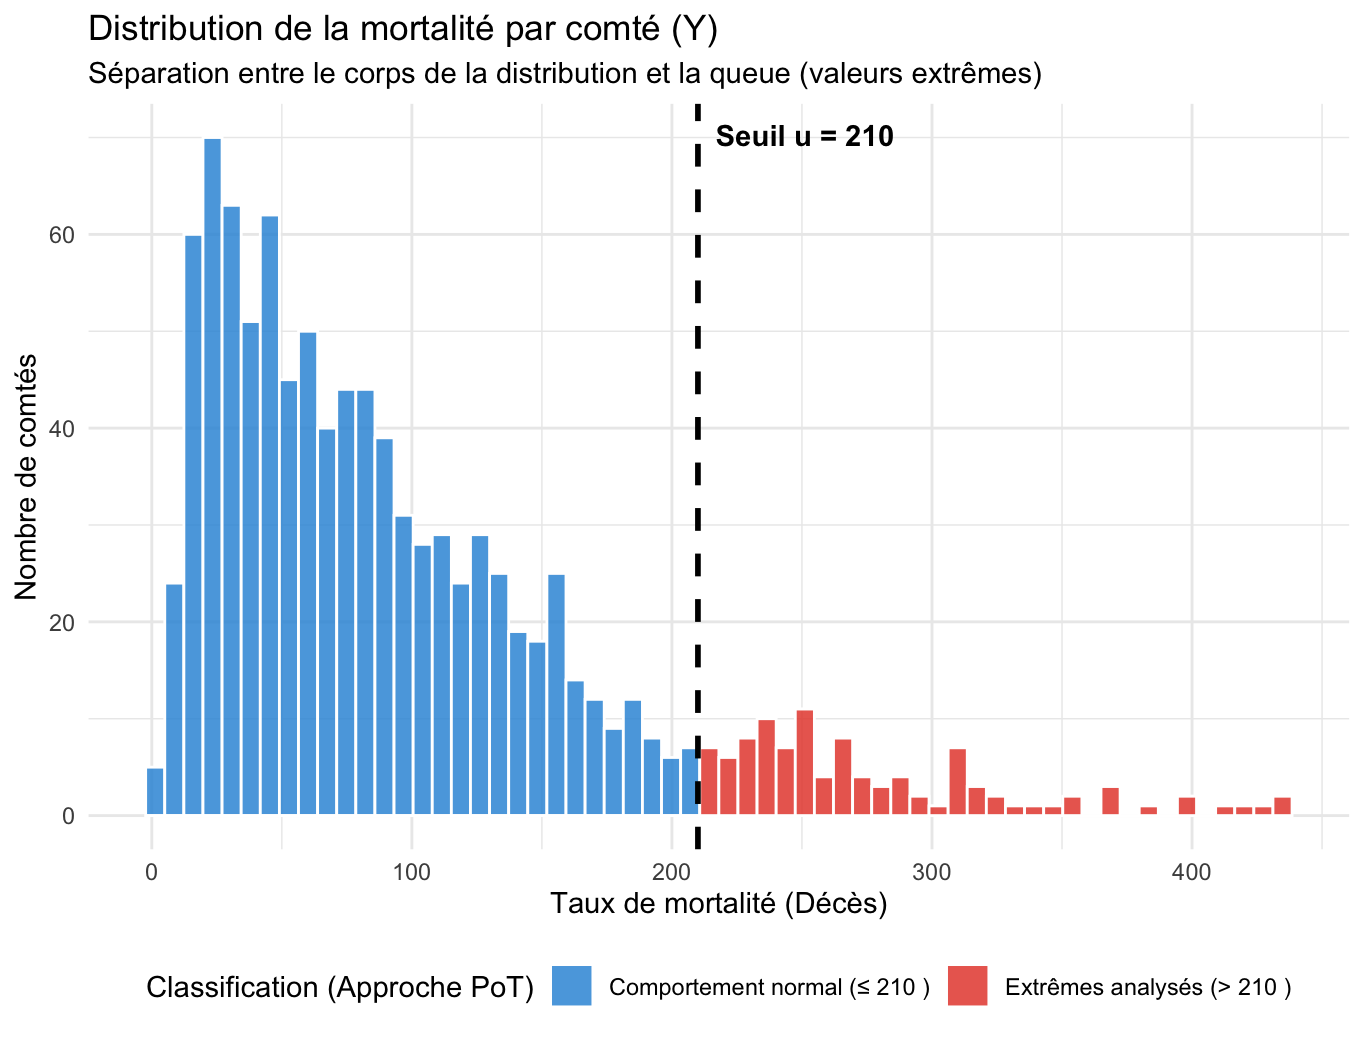
\includegraphics[width=0.38\textwidth]{histogramme1.png}
    \caption{Distribution du taux de mortalité (Y) par comté. La ligne rouge indique le seuil des extrêmes choisi ultérieurement.}
\end{figure}

    \vspace{0.3cm}

    \begin{itemize}
        \item Distribution asymétrique, queue à droite marquée
        \item Seuil d'extrême déterminé par MRL plot $\rightarrow$ slide suivante
    \end{itemize}
\end{frame}

% ---------------------------------------------------
% SLIDE 7 : L'ARBRE DE DECISION
% ---------------------------------------------------
\begin{frame}{Résultats : La segmentation territoriale}
    \begin{center}
        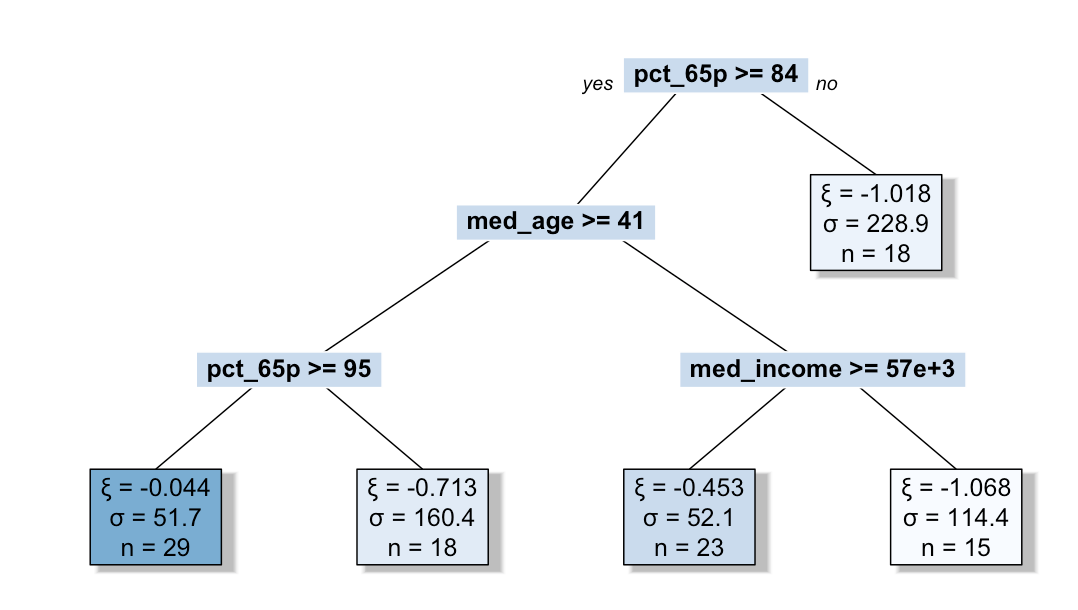
\includegraphics[width=0.55\textwidth]{arbre.png}
    \end{center}
    \vspace{0.2cm}
    \textbf{Lecture de l'arbre :} Le modèle sépare structurellement les comtés d'abord par la proportion de personnes âgées (\texttt{pct\_65p}), puis par la densité urbaine (\texttt{density}).
\end{frame}

% ---------------------------------------------------
% SLIDE 8 : INTERPRETABILITE ET VALIDATION (AIC/BIC)
% ---------------------------------------------------
\begin{frame}{Choix du seuil $u$}
    \textbf{Compromis biais / variance}
    \begin{itemize}
        \item $u$ bas $\rightarrow$ biais (approximation invalide)
        \item $u$ haut $\rightarrow$ variance (échantillon réduit)
    \end{itemize}

    \vspace{0.4cm}

    \textbf{Outil : Mean Residual Life plot}
    \[
    \mathbb{E}[Y - u \mid Y > u] = \frac{\sigma_u}{1 - \xi} + \frac{\xi u}{1 - \xi} \quad \text{(linéaire en } u\text{)}
    \]

    \vspace{0.4cm}

    \begin{itemize}
        \item Linéarité sur $u \in [200, 250]$
    \end{itemize}

    \vspace{0.2cm}

    \begin{center}
    \begin{tcolorbox}[colback=pontsred!10, colframe=pontsred, width=0.4\textwidth]
        \centering \textbf{Seuil retenu : $u = 210$}
    \end{tcolorbox}
    \end{center}
\end{frame}

\begin{frame}{MRL Plot}
    \begin{figure}[H]
    \centering
    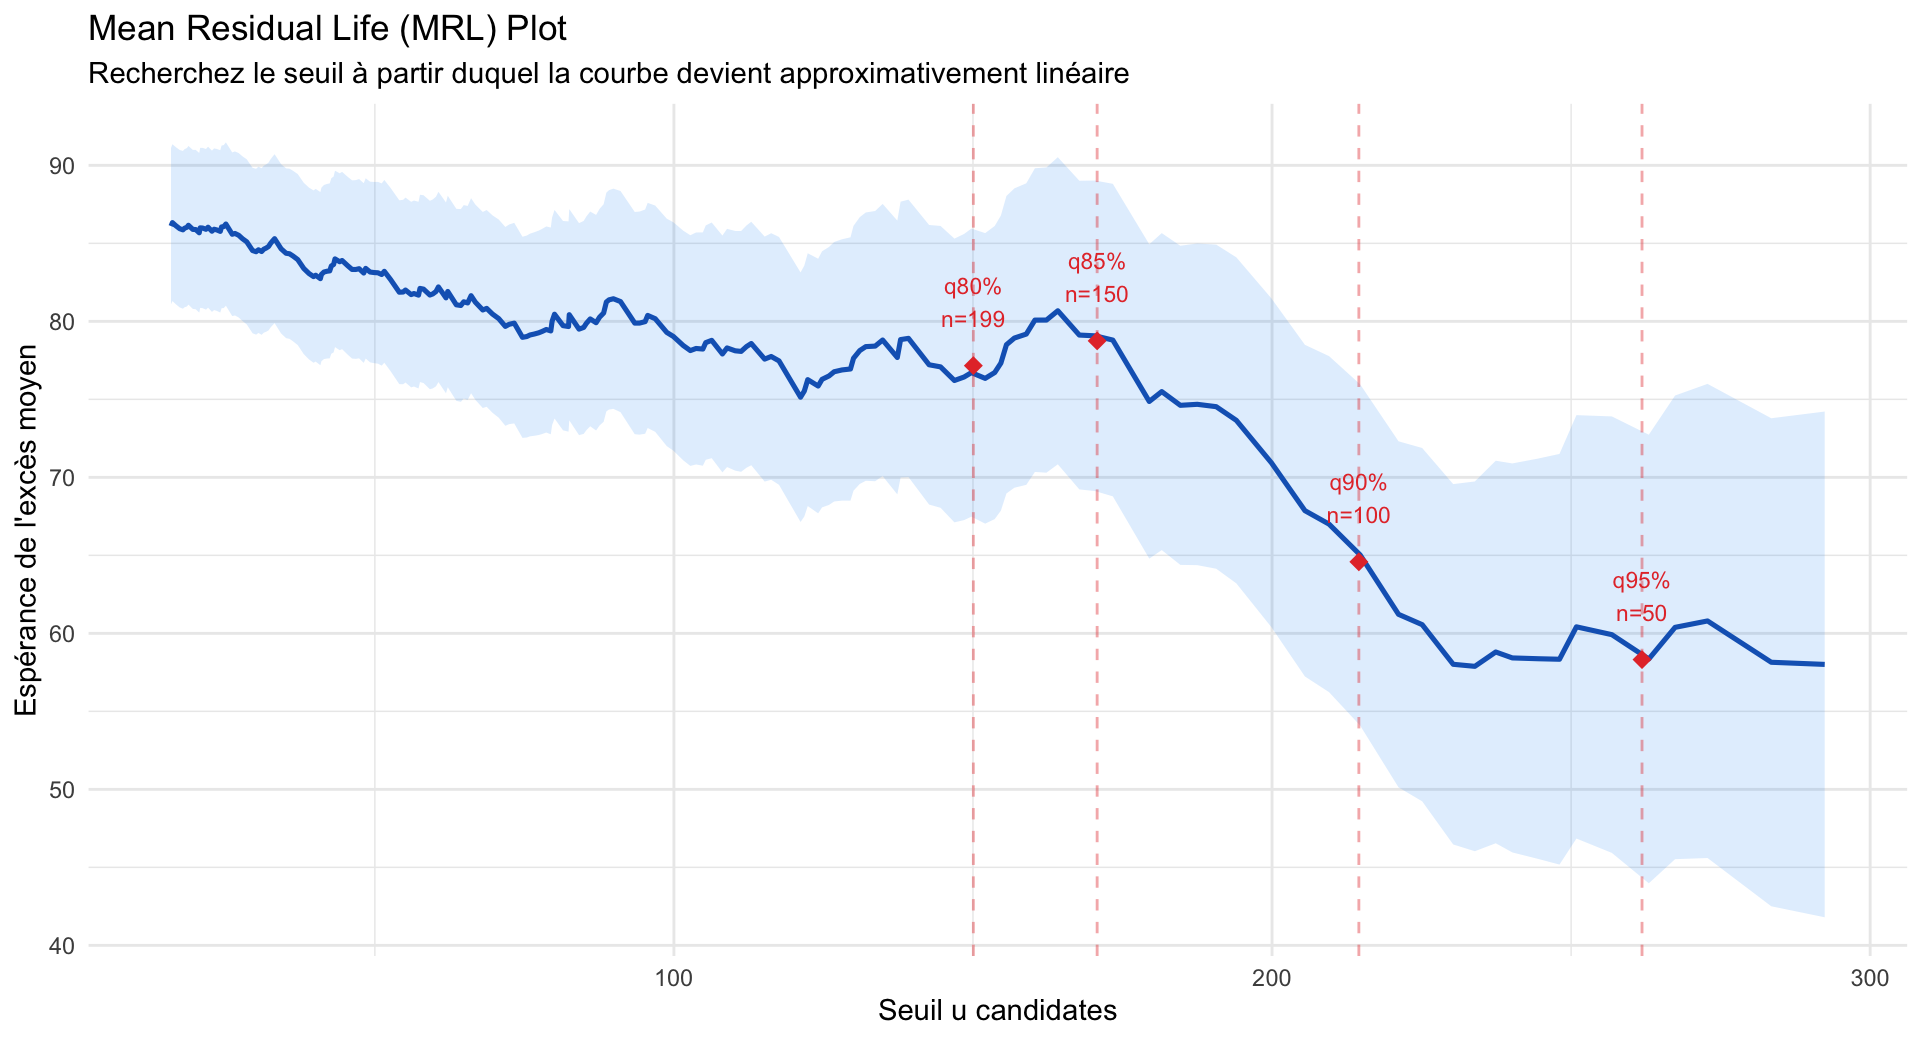
\includegraphics[width=0.5\textwidth]{mrl1.png}
    \caption{Mean Residual Life Plot. La linéarité valide théoriquement l'adéquation d'une GPD au-dessus de 210.}
\end{figure}
\end{frame}

\begin{frame}{Stabilité des paramètres}
    \textbf{Propriété GPD} (Coles, 2001) -- pour $u > u_0$ :
    \[
    \xi_u = \xi_{u_0}, \qquad 
    \]

    \vspace{0.4cm}

    \textbf{Diagnostic} : zones horizontales sur le tracé empirique de $\hat\xi$ par rapport à u

    \vspace{0.4cm}

    \begin{alertblock}{Difficulté}
        \begin{itemize}
            \item Dérive de $\hat\xi$ aux très hauts seuils
            \item $\rightarrow$ IC 95\%
            \item $\hat\xi$ reste dans l'IC autour de $u \approx 200-250$
        \end{itemize}
    \end{alertblock}

    \vspace{0.3cm}

    \centering
    \textit{Hétérogénéité nationale $\Rightarrow$ besoin de partitionner.}
\end{frame}

\begin{frame}{Stabilité de $\xi$}
\begin{figure}[H]
    \centering
    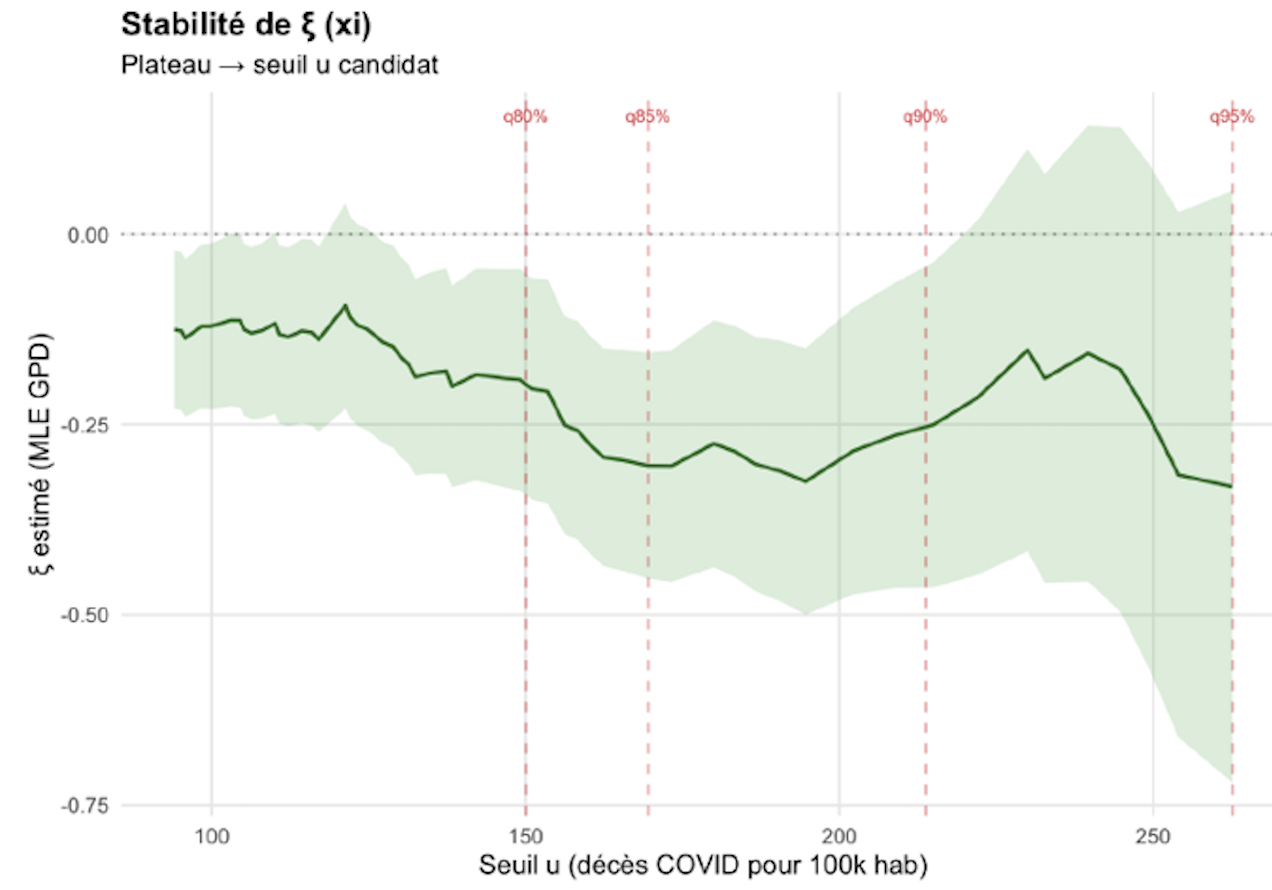
\includegraphics[width=0.6\textwidth]{stabilite.png}
    \caption{Stabilité asymptotique de $\xi$ (avec intervalle de confiance).}
\end{figure}
\end{frame}

% ============================================================
\section{EVT-CART}
% ============================================================


\begin{frame}{Arbre de référence}
    \begin{columns}
        \column{0.25\textwidth}
        \textbf{Variables retenues}
        \begin{itemize}
            \item \texttt{pct\_65p}
            \item \texttt{density}
            \item \texttt{lon}, \texttt{lat}
            \item \texttt{med\_income}
        \end{itemize}

        \vspace{0.2cm}

        \textbf{Sortie}
        \begin{itemize}
            \item 5 feuilles
            \item AIC = 10\,392
        \end{itemize}

        \column{0.7\textwidth}
        \begin{figure}[H]
        \centering
           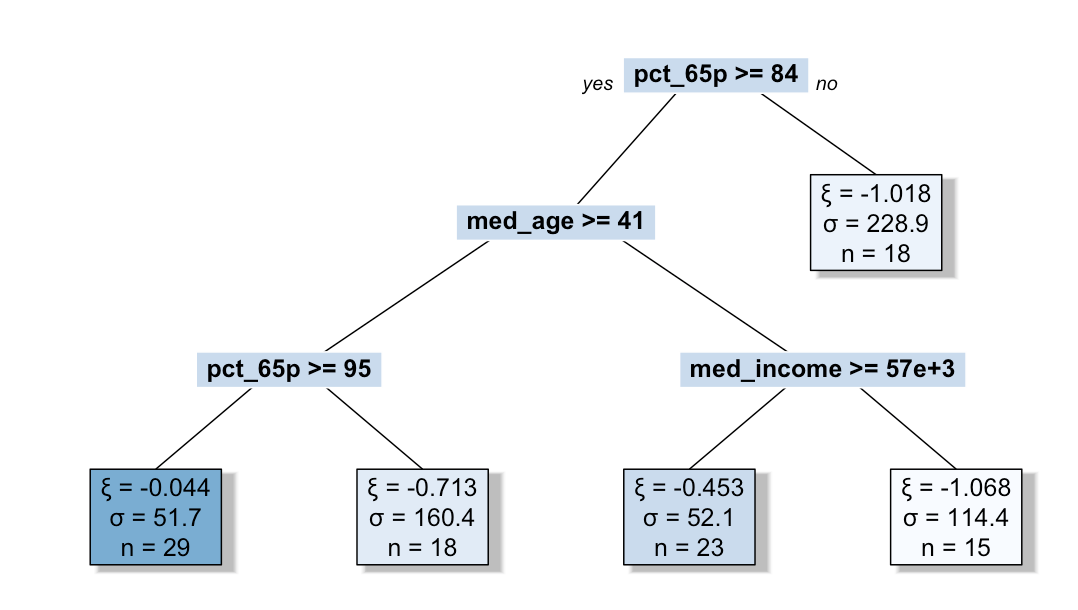
\includegraphics[width=\textwidth]{arbre.png}
            \caption{Arbre EVT-CART ajusté sur les comtés extrêmes.}
        \end{figure}
    \end{columns}
\end{frame}

% ============================================================
\section{Diagnostic}
% ============================================================

\begin{frame}{Diagnostic local -- QQ-plots}
    \begin{columns}
        \column{0.25\textwidth}
        \textbf{3 feuilles / 5} -- succès
        \begin{itemize}
            \item QQ-plots alignés
            \item $\hat\xi < 0$ $\rightarrow$ borne physique
        \end{itemize}

        \vspace{0.4cm}

        \textbf{Feuilles 10 et 11} -- anomalie
        
        \column{0.70\textwidth}
        \begin{figure}[H]
        \centering
        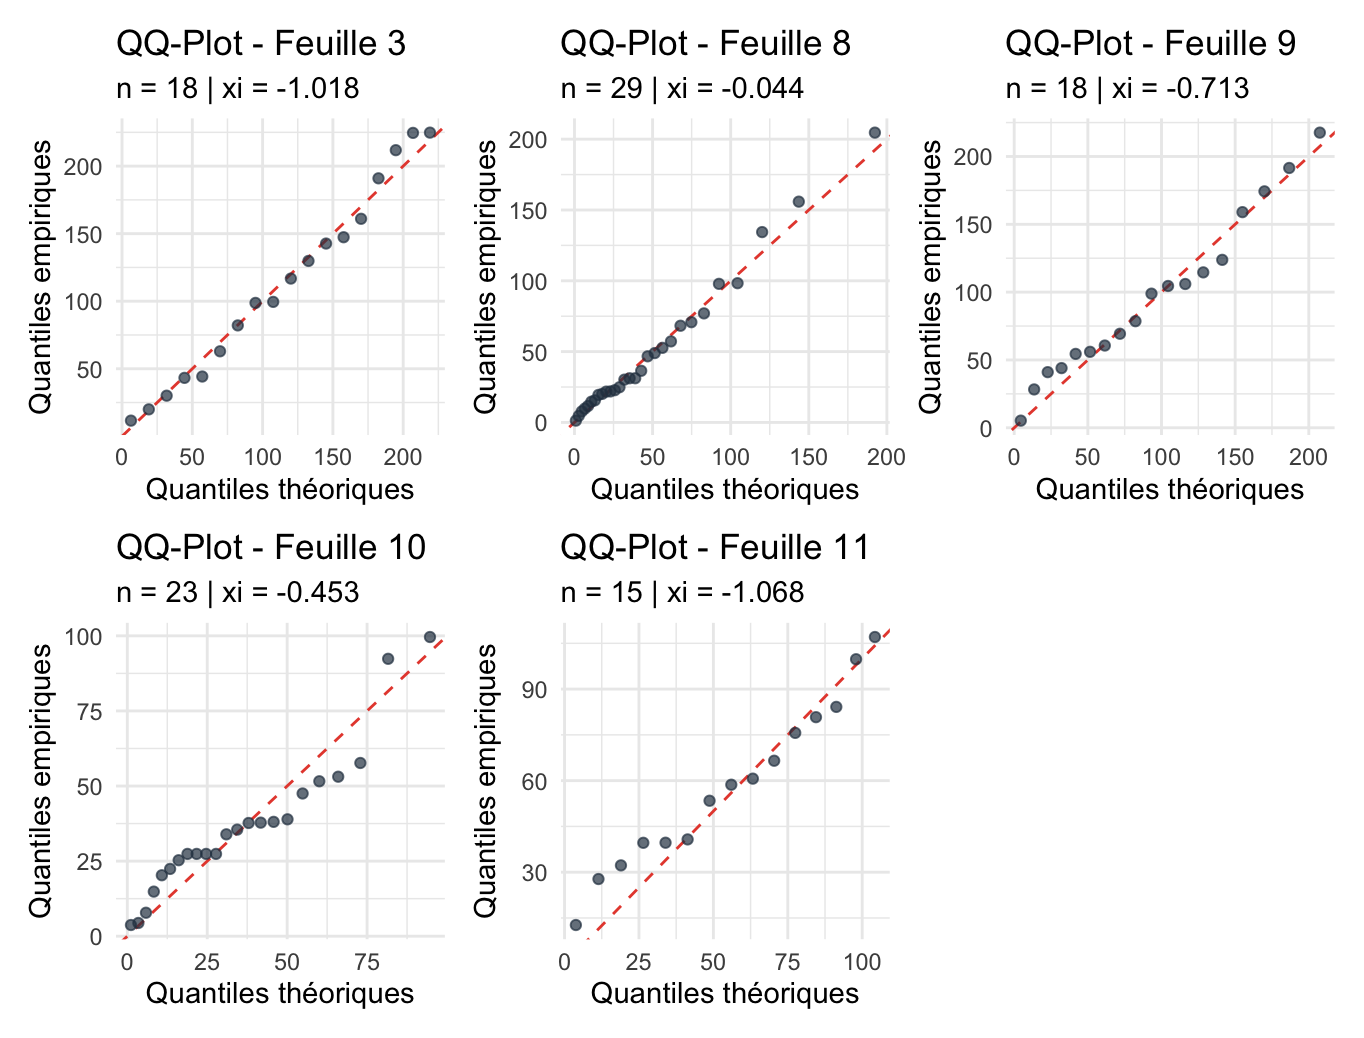
\includegraphics[width=0.8\textwidth]{qq-plots1.png}
        \end{figure}
    \end{columns}
\end{frame}

\begin{frame}{Niveaux de retour}
    \begin{figure}[H]
    \centering
    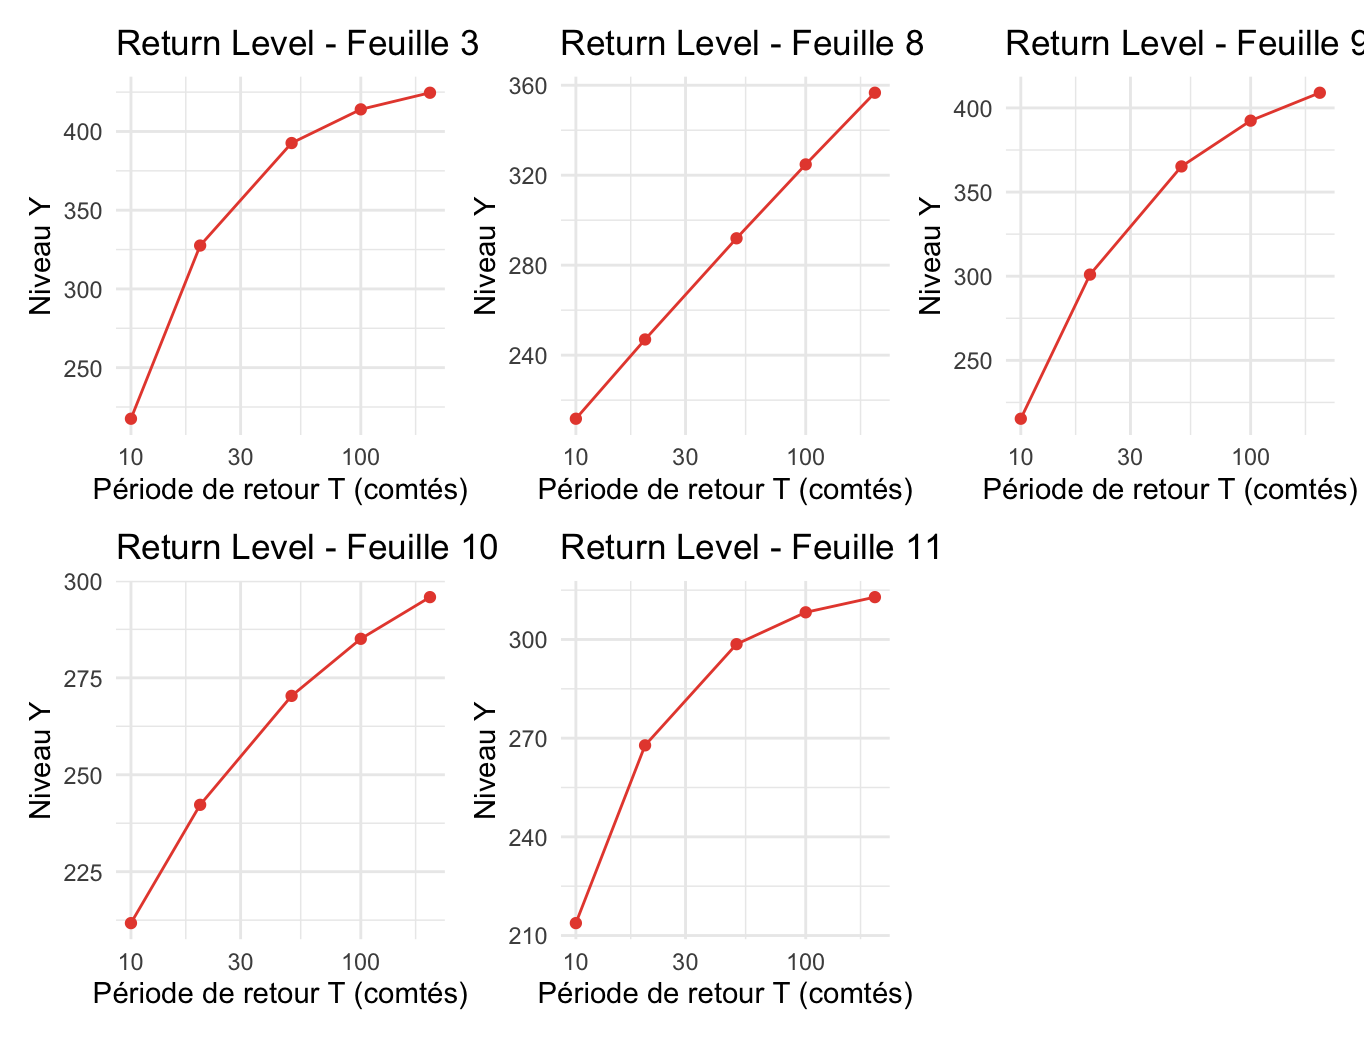
\includegraphics[width=0.48\textwidth]{return1.png}

\end{figure}

    \vspace{0.1cm}

    \begin{itemize}
        \item Courbes concaves $\rightarrow$ $\xi < 0$ (saturation)
        \item Outil de quantification du « pire scénario centennal » par cluster
    \end{itemize}
\end{frame}

% ============================================================
\section{Améliorations}
% ============================================================

\begin{frame}{Ajout de variables socio-économiques}
    \textbf{Variables ajoutées}
    \begin{itemize}
        \item Socio : \texttt{pct\_poverty}, \texttt{pct\_vaccinated}, \texttt{pct\_uninsured}, \texttt{rucc}
        \item Volume : \texttt{population}, \texttt{total\_deaths}, \texttt{deaths\_male}
    \end{itemize}

    \vspace{0.3cm}

    \textbf{AIC} : $10\,392 \rightarrow 9\,935$

    \vspace{0.4cm}

    \begin{alertblock}{Résultat surprenant}
        Splits \textbf{exclusivement} sur les comptages bruts $\rightarrow$ socio-éco ignoré
    \end{alertblock}

    \vspace{0.3cm}

    \textbf{Explication}
    \begin{itemize}
        \item Comptages : variables très proches de la construction du taux
        \item Ratios : information plus indirecte
    \end{itemize}
\end{frame}

\begin{frame}{(b) Suppression des variables corrélées à la cible}
    \textbf{Motivation}
    \begin{itemize}
        \item Éviter la reconstruction triviale de $Y$
        \item Forcer des \textbf{facteurs structurels}
    \end{itemize}

    \vspace{0.4cm}

    \textbf{Résultat}
    \begin{itemize}
        \item Arbre à \textbf{4 feuilles}
        \item AIC = 10\,187,8
        \item Splits principaux : \texttt{pct\_65p}, \texttt{density}
        \item Feuilles toutes distinctes (test de Kolmogorov--Smirnov)
        \item \textbf{Interprétabilité} cohérente avec la littérature
    \end{itemize}
\end{frame}

\begin{frame}{Comparaison des deux arbres}
    \begin{columns}[T,onlytextwidth]
        % --- Colonne gauche ---
        \column{0.48\textwidth}
        \centering
        \textbf{(a) Modèle enrichi}\\
        {\footnotesize avec comptages bruts}

        \vspace{0.3cm}
        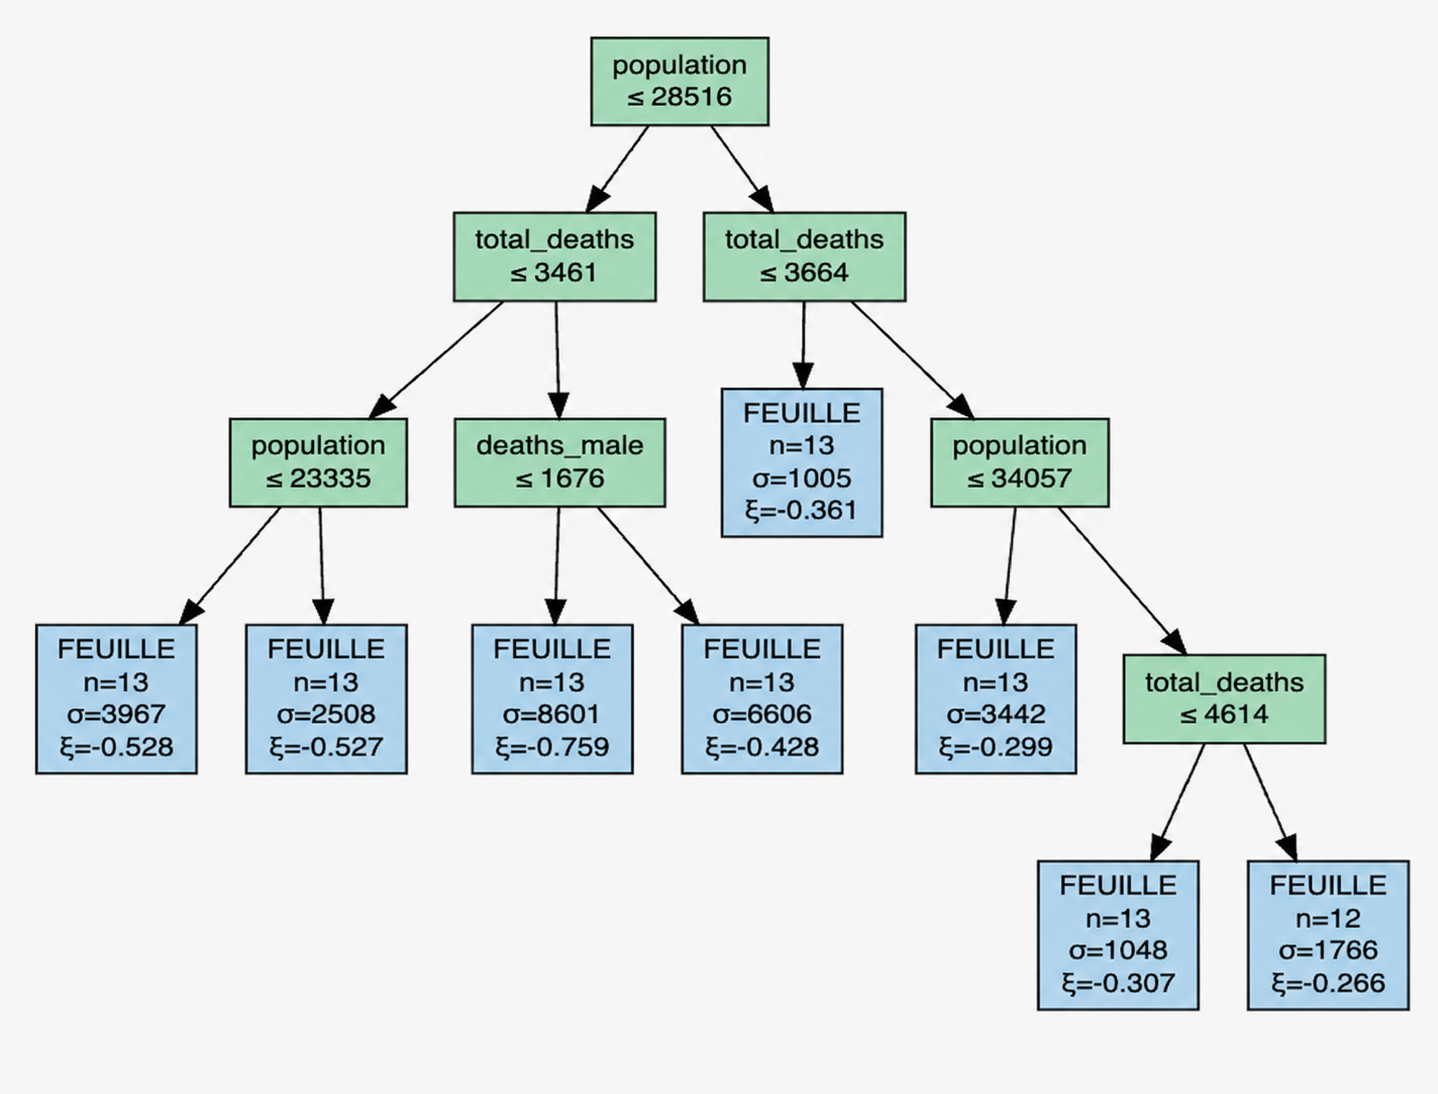
\includegraphics[width=\linewidth,height=0.55\textheight,keepaspectratio]{arbre1.png}

        \vspace{0.3cm}
        \begin{tcolorbox}[colback=pontsblue!10, colframe=pontsblue, boxsep=2pt, left=4pt, right=4pt, top=2pt, bottom=2pt]
            \centering 8 feuilles \quad $\bullet$ \quad \textbf{AIC = 9\,935}
        \end{tcolorbox}

        % --- Colonne droite ---
        \column{0.48\textwidth}
        \centering
        \textbf{(b) Modèle socio-démographique}\\
        {\footnotesize sans variables corrélées à la cible}

        \vspace{0.3cm}
        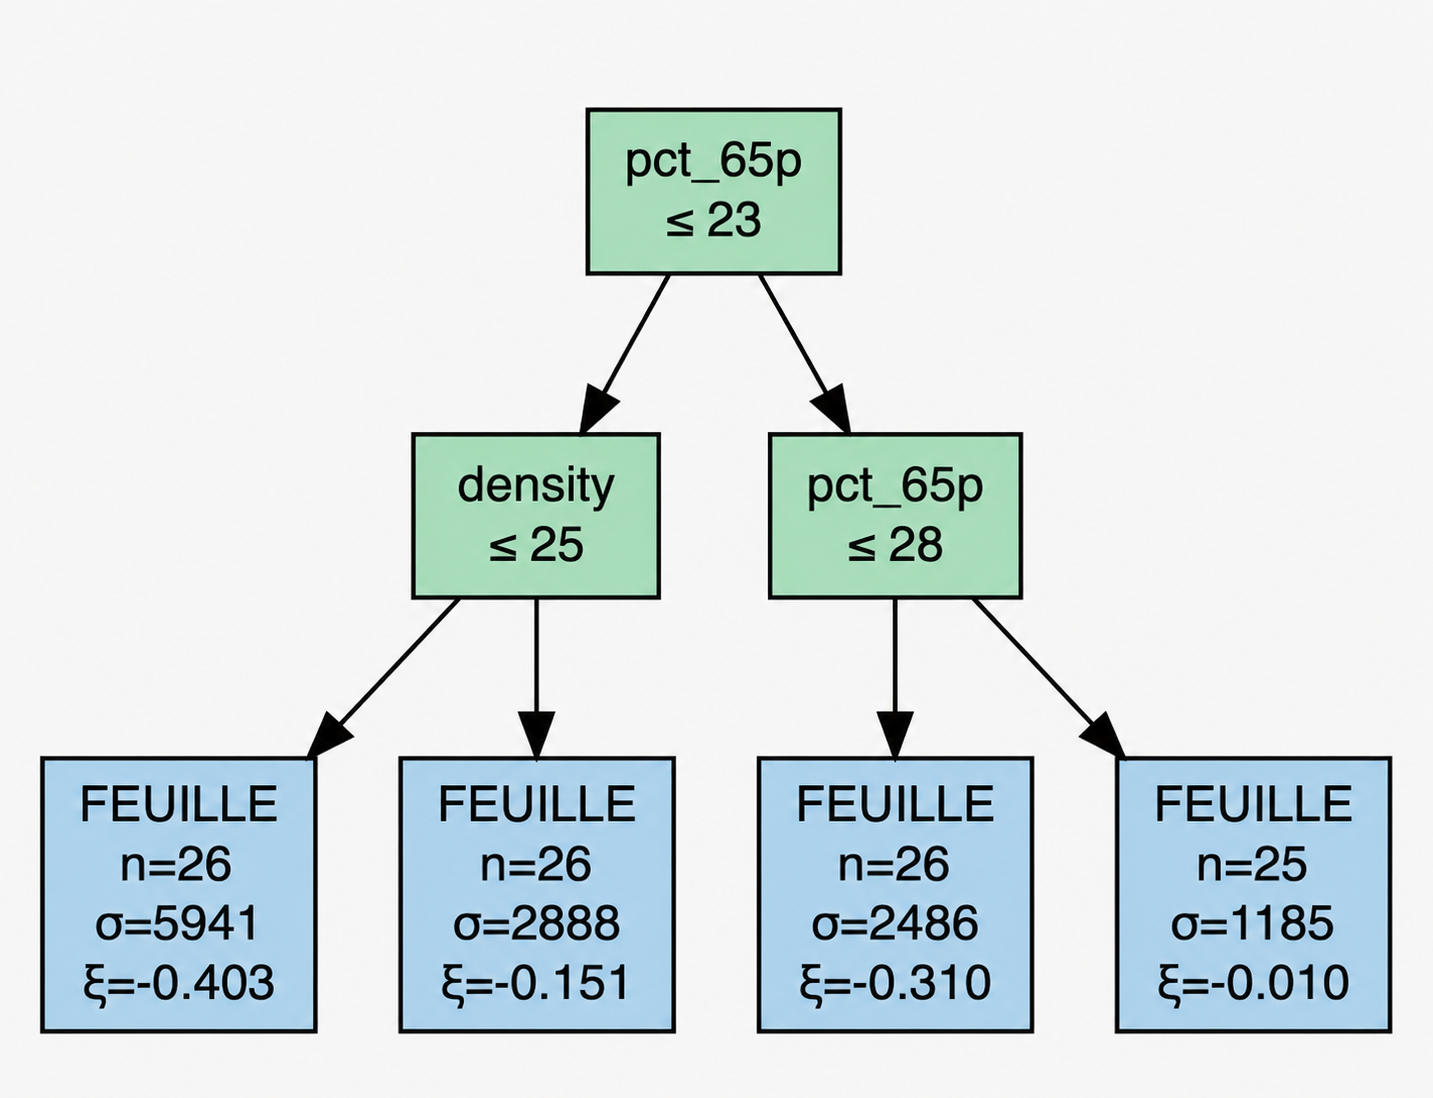
\includegraphics[width=\linewidth,height=0.55\textheight,keepaspectratio]{arbre2.png}

        \vspace{0.3cm}
        \begin{tcolorbox}[colback=pontsred!10, colframe=pontsred, boxsep=2pt, left=4pt, right=4pt, top=2pt, bottom=2pt]
            \centering 4 feuilles \quad $\bullet$ \quad \textbf{AIC = 10\,188}
        \end{tcolorbox}
    \end{columns}

    \vspace{0.4cm}

    \centering
    \footnotesize \textit{Meilleur AIC pour (a), meilleure interprétabilité structurelle pour (b).}
\end{frame}

\begin{frame}{(c) Sensibilité des hyperparamètres}
    \textbf{Hyperparamètres testés}
    \begin{itemize}
        \item \texttt{min\_gain = 5}, \texttt{max\_depth = 4}, \texttt{min\_node = 25}
    \end{itemize}

    \vspace{0.4cm}

    \textbf{Observations}
    \begin{itemize}
        \item \texttt{min\_gain} $<$ 5 $\rightarrow$ aucun split supplémentaire
        \item \texttt{max\_depth} $>$ 4 $\rightarrow$ structure inchangée
        \item \texttt{min\_node} $<$ 25 $\rightarrow$ feuilles non distinctes (KS)
    \end{itemize}

    \vspace{0.4cm}

    \begin{block}{}
        Arbre \textbf{structurellement stable} -- gain min. de 174 points d'AIC vs GPD global
    \end{block}
\end{frame}
% ---------------------------------------------------
% SLIDE 10 : METHODOLOGIE KRIGEAGE
% ---------------------------------------------------
\begin{frame}{Continuité Spatiale : La stratégie du Krigeage}
    \textbf{L'obstacle industriel :} Les données brutes du CDC présentent des "trous" géographiques (comtés sans remontées fiables). Impossible de fournir une carte lacunaire à un client.
    \vspace{0.3cm}

    \textbf{Notre approche hybride pour une carte continue :}
    \begin{enumerate}
        \item \textbf{Top-Down (L'Arbre) :} Les comtés connus passent dans l'EVT-CART et héritent du paramètre de risque extrême ($\xi$) de leur profil social.
        \item \textbf{Bottom-Up (Krigeage) :} Pour les comtés manquants, on interpole $\xi$. Au lieu d'une moyenne naïve, le krigeage ordinaire modélise la corrélation spatiale exacte via un \textit{variogramme}.
    \end{enumerate}
\end{frame}

% ---------------------------------------------------
% SLIDE 11 : LA CARTE FINALE
% ---------------------------------------------------
\begin{frame}[plain]{Livrable Décideur : Cartographie du Risque Extrême ($\xi$)}
    \begin{center}
        \vfill
        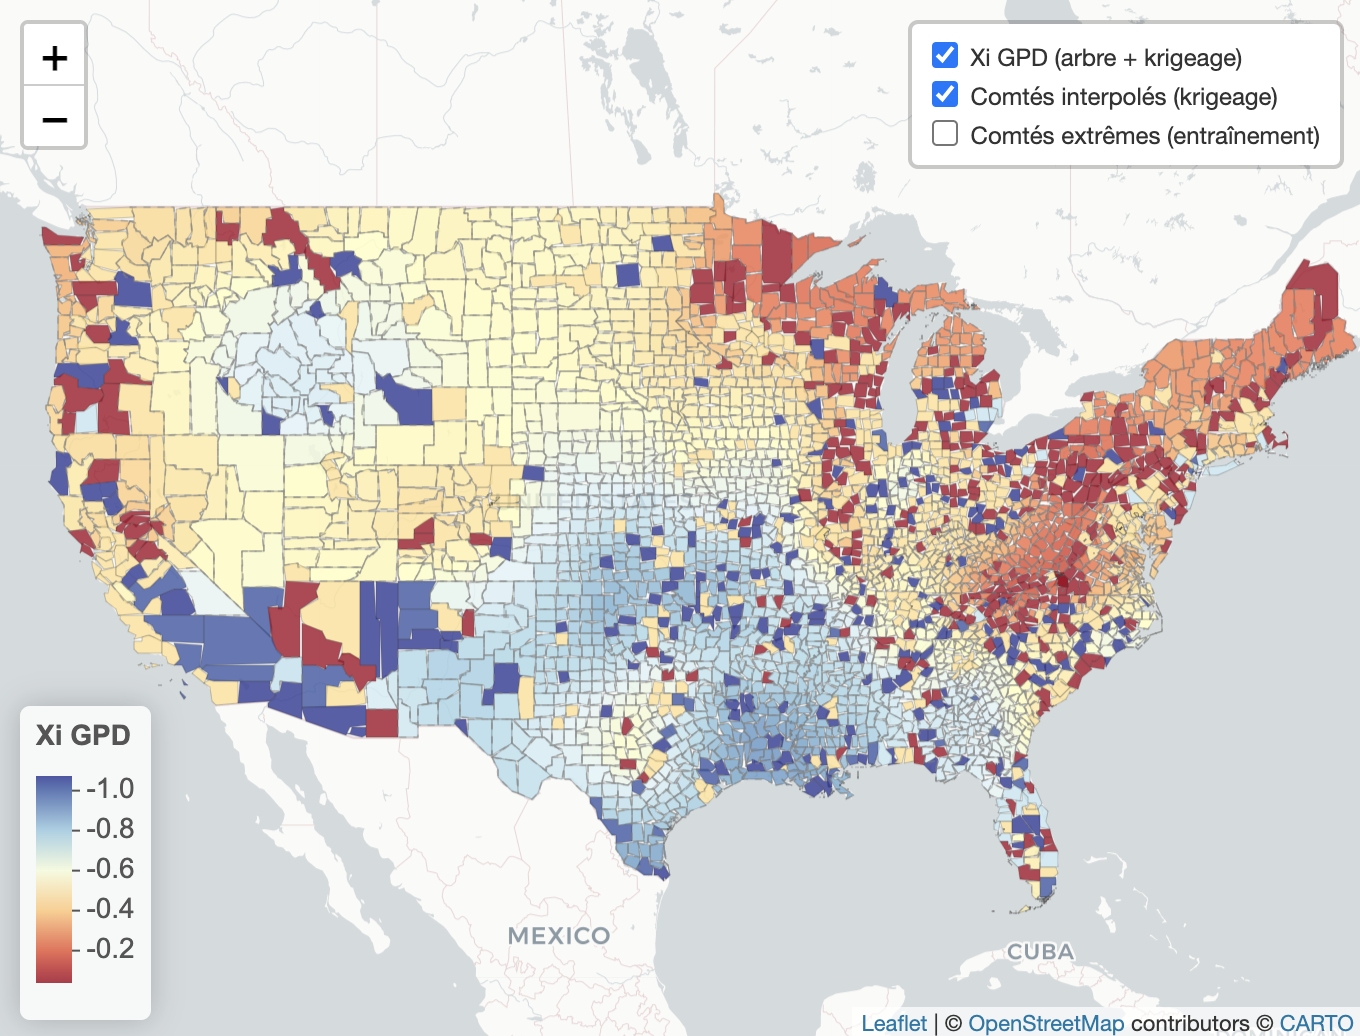
\includegraphics[width=0.9\textwidth, height=0.85\textheight, keepaspectratio]{carte1.png}
        \vfill
    \end{center}
\end{frame}

% ---------------------------------------------------
%  WEB APP (DÉMO VISUELLE)
% ---------------------------------------------------
\begin{frame}{Outil Opérationnel : Interface Interactive RShiny}
    \begin{center}
        \vfill
        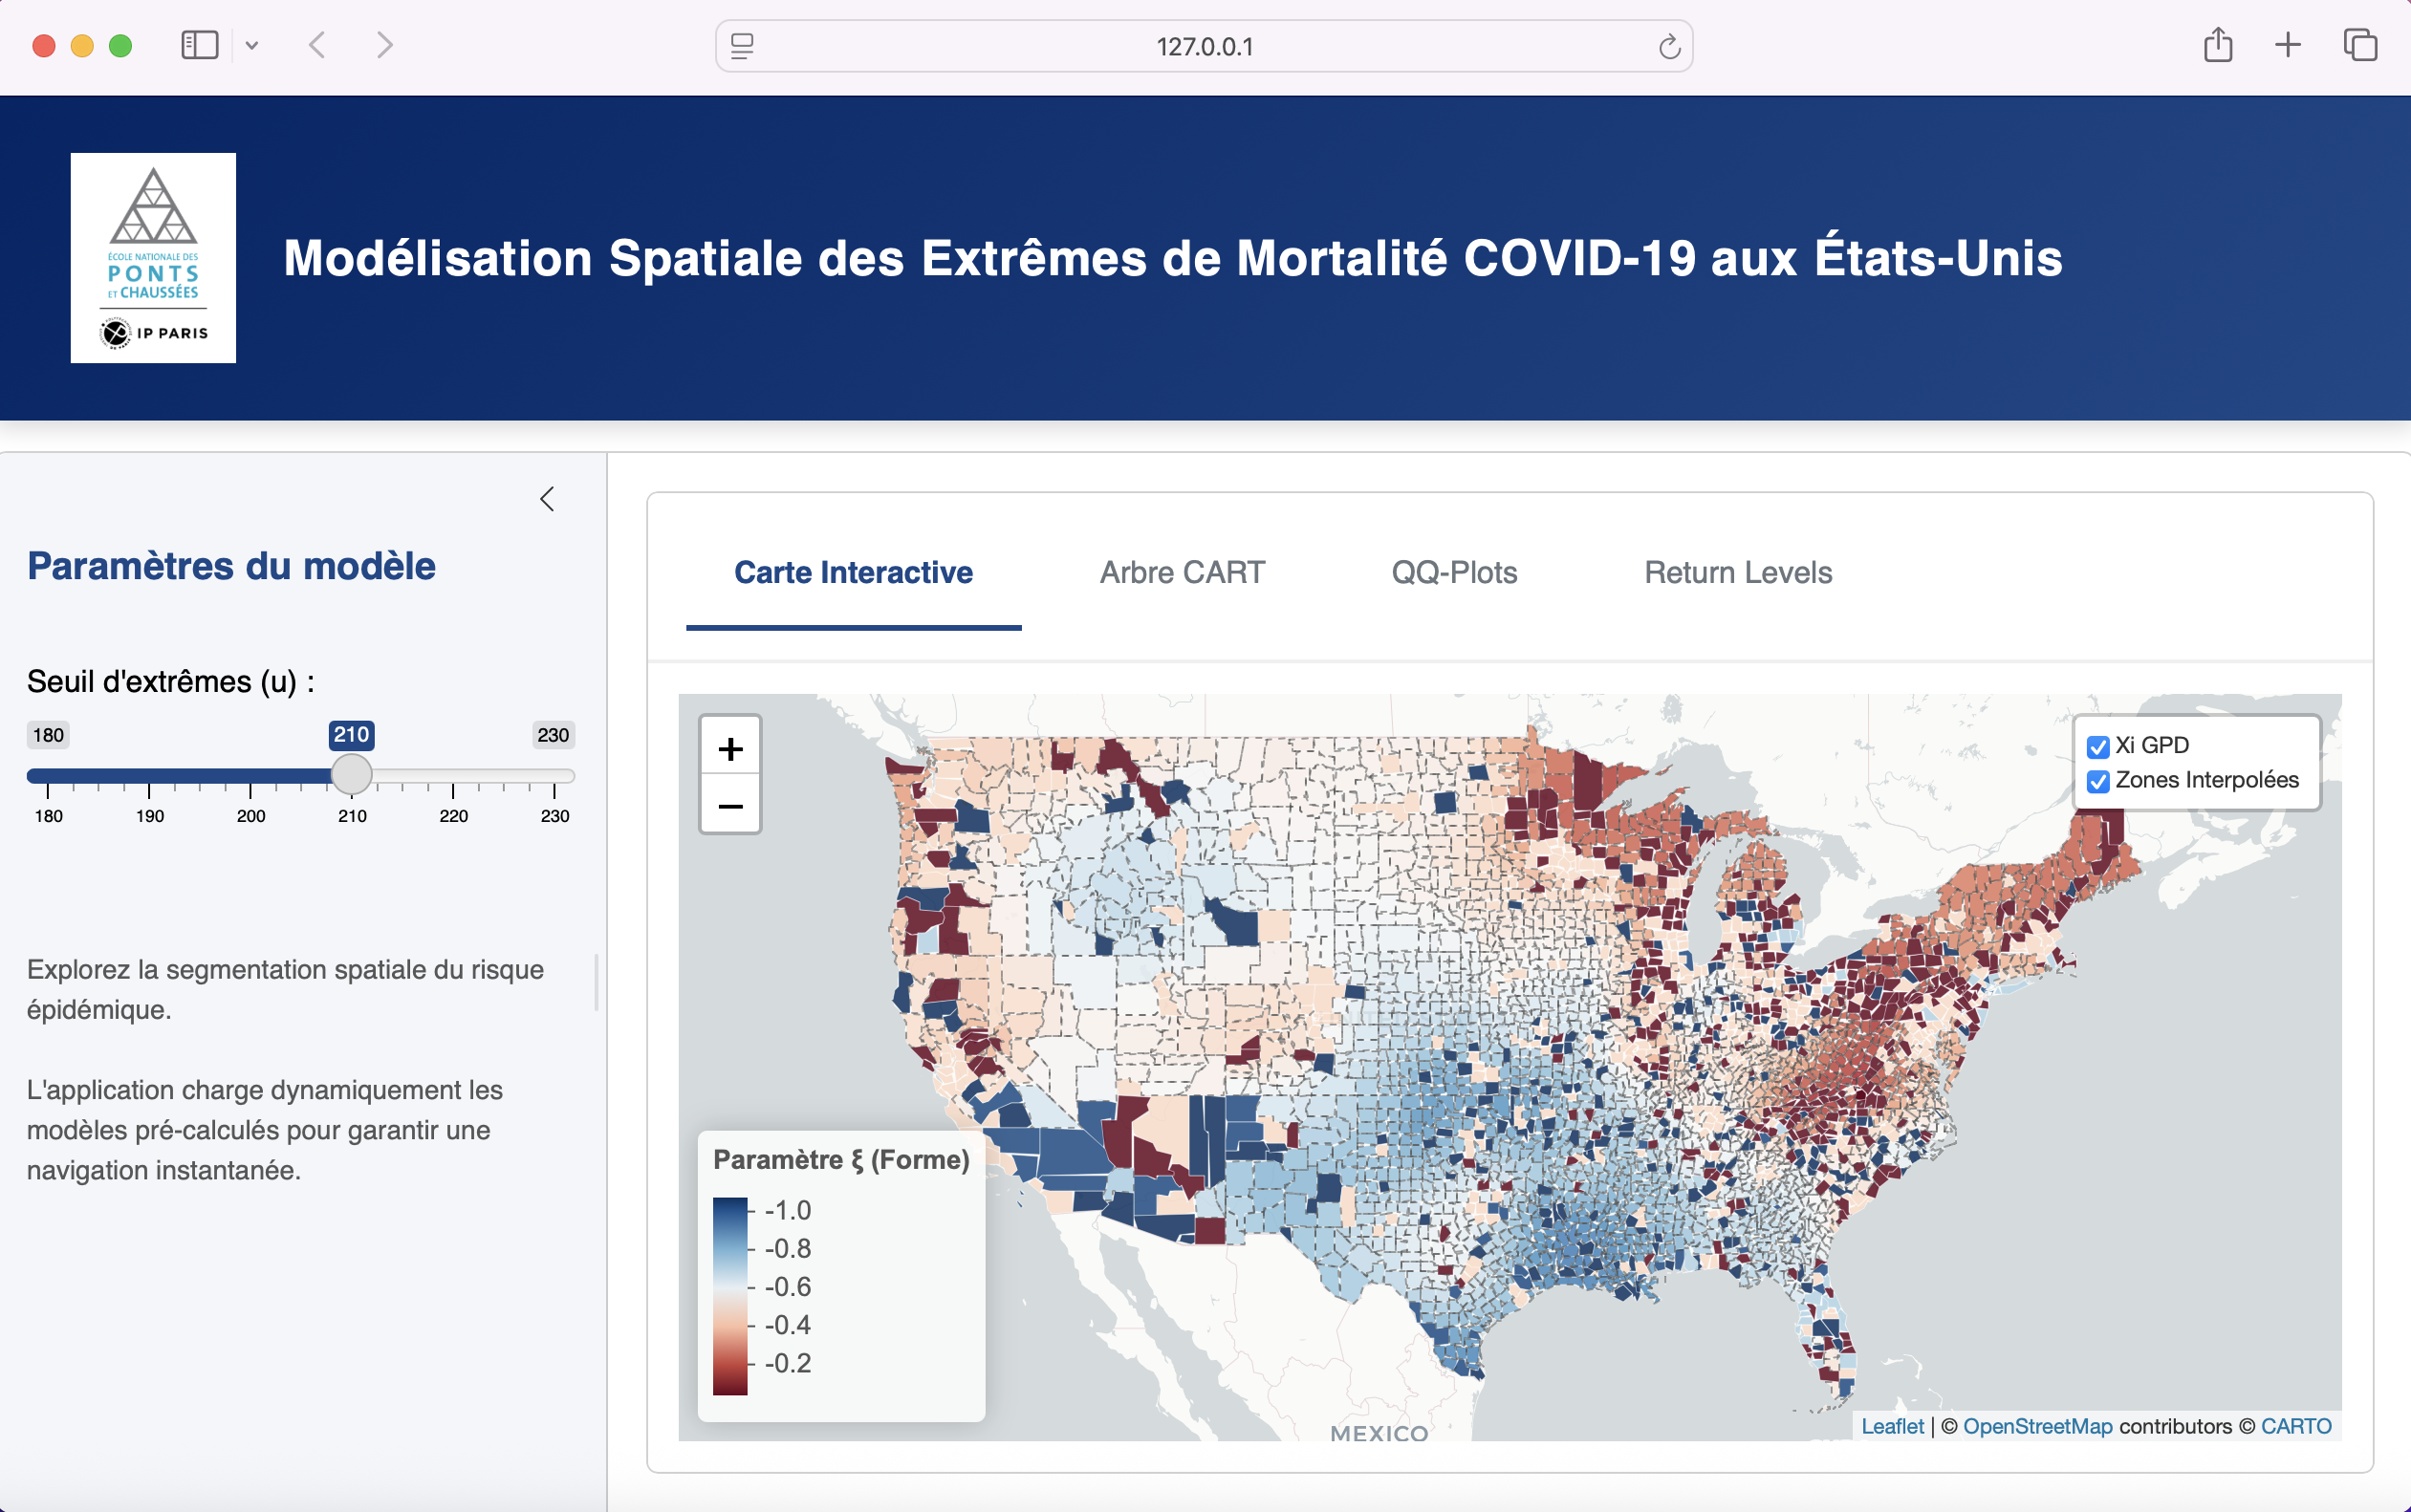
\includegraphics[width=0.95\textwidth, height=0.75\textheight, keepaspectratio]{webapp.png}
        \vfill
    \end{center}
\end{frame}
% ---------------------------------------------------
% SLIDE 12 : CONCLUSION
% ---------------------------------------------------
\begin{frame}{Conclusion et Recommandations Opérationnelles}
    \textbf{Observations Spatiales (Diagnostic)}
    \begin{itemize}
        \item \textbf{Zones d'alerte (Est, Nord et Ouest) :} Le risque d'emballement ($\xi$ plus proche de zéro) est corrélé aux fortes densités et aux populations vieillissantes.
        \item \textbf{Zones tampon (Sud/Centre) :} Le risque y est physiquement "borné" ($\xi < 0$), réduisant la probabilité de saturation systémique.
    \end{itemize}
    \vspace{0.3cm}

    \textbf{Actionnabilité pour le Commanditaire}
    \begin{itemize}
        \item \textbf{Allocation ciblée :} Les splits clés de notre modèle prouvent que la densité (\texttt{density}) et la gériatrie (\texttt{pct\_65p}) sont les vrais moteurs du risque extrême. L'allocation de lits de réanimation d'urgence doit cibler ces zones en priorité absolue.
        \item \textbf{Provisionnement :} L'outil permet de tarifer le risque pandémique localement (Assurance) plutôt que d'utiliser une moyenne nationale trompeuse.
    \end{itemize}
\end{frame}

% ---------------------------------------------------
% SLIDE 13 : Q&A
% ---------------------------------------------------
\begin{frame}[plain]
    \begin{center}
        \vspace{2cm}
        {\Huge \textbf{Merci.}}\\[1cm]
        {\Large Place aux questions.}
    \end{center}
\end{frame}

% ----- References -----
\begin{frame}{Références}
    \footnotesize
    \begin{itemize}
        \item[--] Coles, S. (2001). \textit{An Introduction to Statistical Modeling of Extreme Values}. Springer.
        \item[--] Thomas, M. (2022). \textit{Contributions à la TVE et à la gestion du risque}. Sorbonne Université.
        \item[--] Farkas, Heranval, Lopez \& Thomas (2021). \textit{Generalized Pareto Regression Trees for extreme events analysis}. arXiv:2112.10409.
    \end{itemize}
\end{frame}

\end{document}
